\begin{event}{Workshop on interfacing (math) software with low level libraries}{Cernay 2018}{Cernay (France) 2018-04-30 to 2018-05-04}{PS,UV,UG,LL,UB}{24}{11}{https://github.com/OpenDreamKit/OpenDreamKit/issues/251}

  \textbf{Main goals.} This developer meeting was focused on
  initiating long term work on ODK tasks related to packaging,
  portability and documentation tools for SageMath.

  \textbf{ODK implication.} This event was organized and funded by
  \ODK (Paris Sud, \approx 6k€).

  \textbf{Event summary.} An intensive week with some short informal
  presentations, and many brainstorms and coding sprints.

  \textbf{Demographic.} 11 ODK participants from five sites together
  with 14 other experts of a variety of systems such as Oscar,
  Polymake, CERN's Root, Cython, Jupyter and C++, Numba, Dask,
  libsemigroups.

  \textbf{Results and impact.} (Math) Computational systems face a
  tension between using high level languages (e.g. Python) for
  expressivity, ease of use and prototyping, and low-level languages
  (e.g. C/C++) for power and speed, and also for modularity (using
  existing libraries, or writing reusable ones). To resolve this
  tension, many approaches have been explored in the recent years, and
  the frontier between the two worlds is becoming increasingly blurry.

  This workshop brought together developers from a large variety of
  horizons to share expertise, seek collaboration venues, and get into
  concrete action. This was quite bold of an aim.

  Nevertheless, thanks to an informal and flexible format the week
  ended up being very productive, as testified by the progress reports
  and exit survey: to the question “Would you recommend to your
  colleagues to attend a workshop with this format”, 9 answers were
  ``yes definitely'' ad the other two ``yes''; a participant well
  outside of ODK's usual scope wrote as testimony «The looseness made
  it more productive than any workshop I've ever attended».

  Notes were taken collectively with the eventual aim to author a
  joint survey of the available technologies and best practices; the
  current draft is available from
  \url{https://www.overleaf.com/read/wrmkhfvwmxnz}.

  \begin{figure}[ht]
    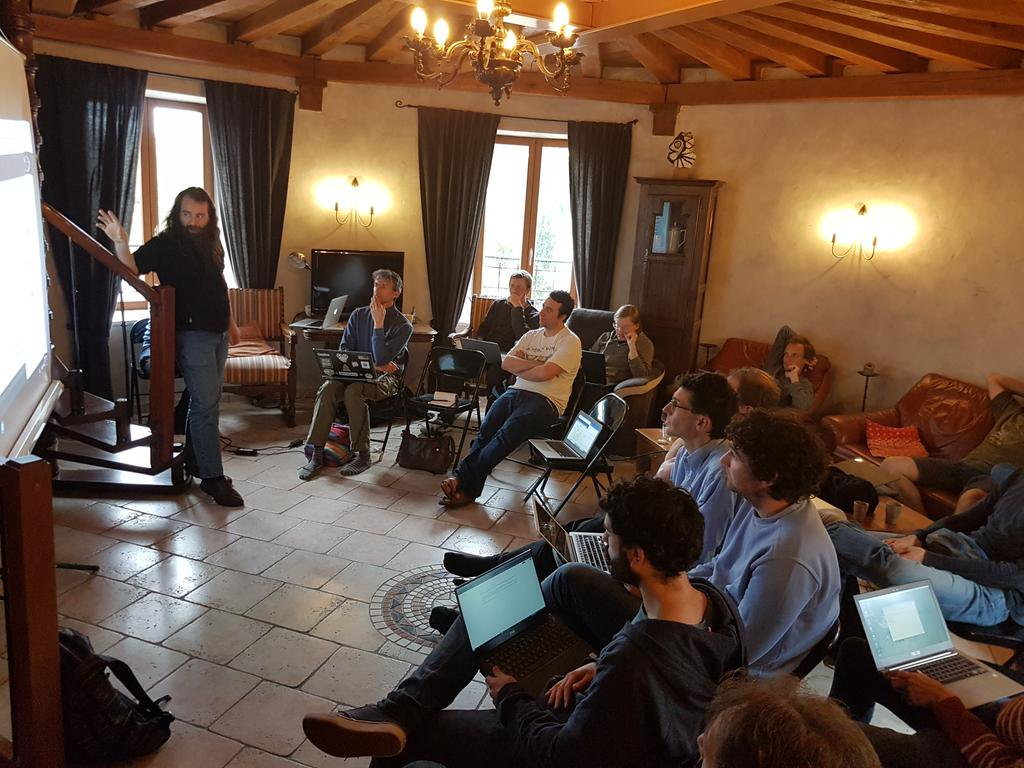
\includegraphics{2018-04-30-Cernay.jpg}
    \caption*{Jim Pivarski, CERN Root developer, presenting on columnar
      storage for HPC in the context of data analysis for high-energy
      physics}
  \end{figure}

\end{event}
